\documentclass[a4paper,twoside]{article}

\usepackage[utf8]{inputenc}
\usepackage[ngerman]{babel}
\usepackage{url} %Bib
\usepackage[sort&compress,numbers]{natbib} %Bib
\usepackage{float}
\usepackage{cuted}
\usepackage{epsfig}
\usepackage{subfigure}
\usepackage{calc}
\usepackage{amssymb}
\usepackage{amstext}
\usepackage{amsmath}
\usepackage{amsthm}
\usepackage{multicol}
\usepackage{pslatex}
\usepackage{apalike}
\usepackage{enumitem}
\usepackage{etoolbox}
\usepackage{hyperref}
\apptocmd{\UrlBreaks}{\do\f\do\m}{}{}
\usepackage{MOSI}     % Please add other packages that you may need BEFORE the MOSI.sty package.

\newcommand{\team}{Patrick Neher, Ruedi Lüthi}
\newcommand{\theme}{Golfstrom}
\setcounter{page}{1}

\subfigtopskip=0pt
\subfigcapskip=0pt
\subfigbottomskip=0pt

\begin{document}

	\title{Der Golfstrom\subtitle{ein mathematisches Modell} }
	
	\author{\authorname{Patrick Neher und Ruedi Lüthi}}
	
	\keywords{Golfstorm, Stabilitätsanalyse}

	\abstract{Der Golfstrom strömt. Schnell!!!!!!}
	
	\onecolumn \maketitle \normalsize \vfill

	\section{\uppercase{Der Golfstrom}}\label{sec:Golfstrom}

	\noindent Der Golfstrom ist ein Naturphänomen, welches für einen Wasseraustausch zwischen dem Golf von Mexiko und dem Nordmeer verantwortlich ist. Die Strömung beginnt jedoch nicht erst im Golf vom Mexiko sondern schon davor. Auf der Höhe des Äquator westlich von Afrika wird das Oberflächenwasser stark erwärmt, da dort die Sonne nahezu senkrecht über dem Wasser steht. Dies trägt dazu bei, dass der Albedo-Wert (Wie viel Prozent der auftreffenden Strahlung reflektiert wird) klein wird und somit viel Energie in das Wasser über geht.

	Der Südost-Passat treibt dieses wärmere Wasser dann in Richtung Golf von Mexiko. Dort vereinigt sich der Strom vom Äquator mit dem Floridastrom. Ab dort Sprechen wir vom Golfstrom, den wir auch in unserem Modell betrachten. Im Golf vor Mexiko erwärmt sich das Wasser weiter bis es dann entlang der Küste Amerikas in Richtung Norden zieht. Dort spaltet sich dich Strömung und ein Teil wird von den Nordost-Passat Winden wieder Richtung Äquator gezogen und bildet einen Kreislauf. Dieser wird in unserem Modell jedoch nicht beachtet. Wir untersuchen den Teil der von der Westwindzone erfasst wird und auf dem 45 Breitengrad Richtung Europa gezogen wird.

	Dort Strömt er dann an der Norwegischen Küste weiter nach Norden. Auf dem Weg kühlt sich das warme Wasser vom Süden wieder ab und erwärmt die Luft, die dann durch die Westwinde zu uns kommt und damit unsere Temperatur stark beeinflusst. Aufgrund des Golfstromes ist unsere durchschnittliche Jahrestemperatur rund 5-10 Grad Celsius wärmer als z.B im Kanada auf dem selben Breitengrad. 

	Weiter im Norden kühlt sich das Wasser weiter ab, bis es dann anfängt zu gefrieren. Dabei wird das Salz aus dem Wasser gelöst, da dieses nicht gefriert. Deshalb steigt der Salzgehalt im nicht gefrorenen Wasser. Dies führt dazu, dass sich die Dichte des Wassers erhöht und sich deshalb absenkt. Das gesunkene Wasser fließt dann entlang der amerikanischen Küste wieder zurück zum Golf von Mexiko.
	\begin{figure}[!h]
  		\centering
 		
\includegraphics[width=7cm]{../Diagramme/Golfstrom.jpg}
  		\caption{Darstellung vom Fluss des Golfstromes}
  		\label{fig:flussGolfstrom}
	\end{figure}

Durch den Golfstrom werden maximal 150 Millionen Kubikmeter Wasser in Bewegung gesetzt. 
Die Erwärmung der Luft ist vergleichbar mit der Leistung von Zwei Millionen modernen Atomkraftwerken. (~1.5 Petawatt)
Im Nordmeer fällt das Wasser in eine Tiefe von über 2000 Metern.
 
	

	
	\section{\uppercase{Das Modell}}\label{sec:Modell}
	
	%\noindent In dem mathematischen Modell wird von zwei Behälter ausgegangen, welche sich durch einen Fluss gegenseitig beeinflussen. Dieser Fluss beschreibt den Golfstrom: 	
	
	\noindent Das mathematische Modell besteht aus zwei Behälter \(1,2\). Diese beeinflussen sich jeweils durch den Fluss gegenseitig, gleichzeitig werden sie aber auch von konstanten Umgebungsgrößen der jeweiligen Behälter beeinflusst.
	
	\begin{figure}[!h]
  		\centering
 		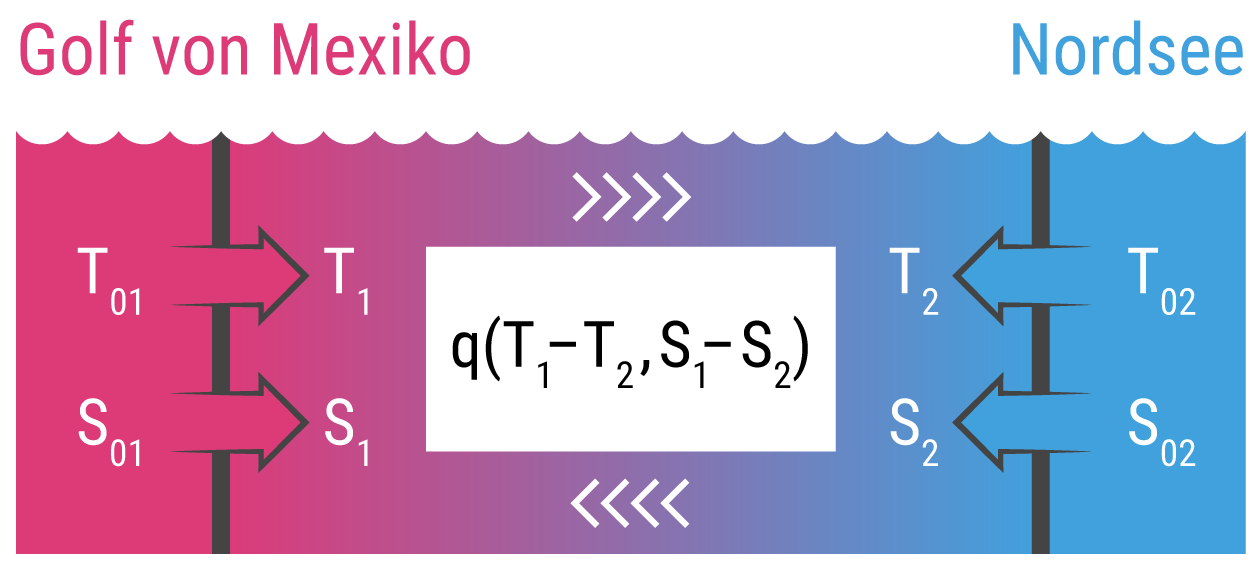
\includegraphics[width=7cm]{../Diagramme/skizze_modell.png}
  		\caption{Schematische Darstellung der zwei Behälter und des Flusses (Golfstrom) dazwischen.}
  		\label{fig:modell}
	\end{figure}
	
	Für die Indexbezeichnung der Variablen gilt in Abbildung \ref{fig:modell} sowie für das ganze nachfolgende Dokument:
	\begin{align*}
		1 &: \textrm{Golf von Mexiko} \\
		2 &: \textrm{Nordsee}
	\end{align*}

	Jeder Behälter \(i\) hat jeweils zwei sich verändernde Variablen:
	\begin{align*}
		T_i &: \textrm{Temperatur} \\
		S_i &: \textrm{Salzgehalt}
	\end{align*}
	
	Die Umgebung der Behälter wird durch folgende Konstanten beschrieben:
	\begin{align*}
		T_{0i} &: \textrm{Temperatur der Umgebung} \\
		S_{0i} &: \textrm{Salzgehalt der Umgebung}
	\end{align*}
	
	Durch das zugrunde liegende physikalische Modell \textbf{???} wird davon ausgegangen, dass sich die Behälter langsam an die Umgebungstemperatur anpassen. Also kann die Veränderung durch die Umgebungsgrößen folgendermaßen mathematisch beschrieben werden:
	\begin{align*}
		\frac{dX_i}{dt} = k_X \left( X_{0i} - X_i \right)
	\end{align*}
	Dabei ist \(X\) die zu verändernde Größe (in unserem Modell entweder \(T\) oder \(S\)).
	Die Veränderung ist also eine Zunahme der Differenz zwischen aktuellem Wert und dem Wert der Umgebung multipliziert mit einer Austauschkonstante \(k_X\).
	
	Wiederum aus dem physikalische Modell ist bekannt, dass die Veränderung durch den Fluss \(q\) sich proportional zur Differenz der Dichte der beiden Behälter beschreiben lässt:
	\begin{align*}
		q = a \left( \rho_2 - \rho_1 \right)
	\end{align*}
	Wie viel Meereswasser nun zwischen den zwei Behälter hin und her fließt, unterliegt sicherlich noch weiteren Umwelteinflüssen. Diese werden in der Konstante \(a\) zusammengefasst.
	
	Die Dichte ist abhängig von Temperatur und Salzgehalt des Meereswasser. Dieser Zusammenhang wird hier vereinfacht als linear angenommen:
	\begin{align*}
		\rho_i = \rho_0 - bT_i + cS_i
	\end{align*}
	
	Die Konstanten \(b\) und \(c\) sind also unveränderliche Naturkonstanten.
	
	Setzt man den Zusammenhang für die Dichte in die Gleichung für den Fluss ein:
	\begin{align*}
		q &= a \left( \rho_0 - bT_2 + cS_2 - \left( \rho_0 - bT_1 + cS_1 \right) \right) \\
		&= a \left( b\left( T_1 - T_2 \right) - c \left( S_1 - S_2 \right) \right)
	\end{align*}
	So wird ersichtlich, dass für den Fluss die Referenzdichte \(\rho_0\) keinen Einfluss hat.
	
	Alles zusammengesetzt ergibt für die vier veränderlichen Größen folgendes Gleichungssystem:
	\begin{align*}
		\frac{dT_1}{dt} &= k_T\left(T_{01} - T_1\right) + \left|q(T_1 - T_2,S_1 - T_2)\right|\left(T_2 - T_1\right) \\
		\frac{dT_2}{dt} &= k_T\left(T_{02} - T_2\right) + \left|q(T_1 - T_2,S_1 - T_2)\right|\left(T_1 - T_2\right) \\
		\frac{dS_1}{dt} &= k_S\left(S_{01} - S_1\right) + \left|q(T_1 - T_2,S_1 - T_2)\right|\left(S_2 - S_1\right) \\
		\frac{dS_2}{dt} &= k_S\left(S_{02} - S_2\right) + \left|q(T_1 - T_2,S_1 - T_2)\right|\left(S_1 - S_2\right)
	\end{align*}
	 
	 In den Gleichungen treten die abhängigen Größen jeweils immer als Differenz der beiden Behälter auf. Also kann das Modell so umgeschrieben werden, dass es nur noch von den Differenzen abhängt. Sei \(T = T_1 - T_2, T_0 = T_{01} - T_{02}\) und \(S = S_1 - S_2, S_0 = S_{01} - S_{02}\)  so ist:
	 \begin{align*}
	 	\frac{dT}{dt} = \frac{dT_1}{dt} - \frac{dT_2}{dt} &= k_T\left(T_{0} - T\right) - 2\left|q(T,S)\right|T \\
	 	\frac{dS}{dt} = \frac{dS_1}{dt} - \frac{dS_2}{dt} &= k_S\left(S_{0} - S\right) - 2\left|q(T,S)\right|S \\
	 	q(T,S) &= a\left(bT - cS\right)
	 \end{align*}
	  
	Aus der Realität \textbf{???} ist bekannt, dass die Umgebungstemperatur \(T_1\) im Golf von Mexiko höher ist als in der Nordsee \(T_2\). Auch bekannt ist, dass der Salzgehalt \(S_1\) im Golf tiefer ist als in der Nordsee \(S_2\). Es gilt also:
	\begin{align*}
		T_1 > T_2 \quad \textrm{und} \quad S_1 < S_2
	\end{align*}
	
	Diese Bedingungen sind in einer ersten Simulation in Abbildung \ref{fig:modell_q_pos} dargestellt. Klar zu erkennen ist, dass sich bereits nach nur kurzer Zeit für den Fluss einen stabilen Zustand einstellt. Der Fluss stellt sich zum Ende bei \(0.45\), also fließt Wasser vom Golf von Mexiko über die Oberfläche in die Nordsee und im Untergrund wieder zurück.
	
	\begin{figure}[!h]
  		\centering
 		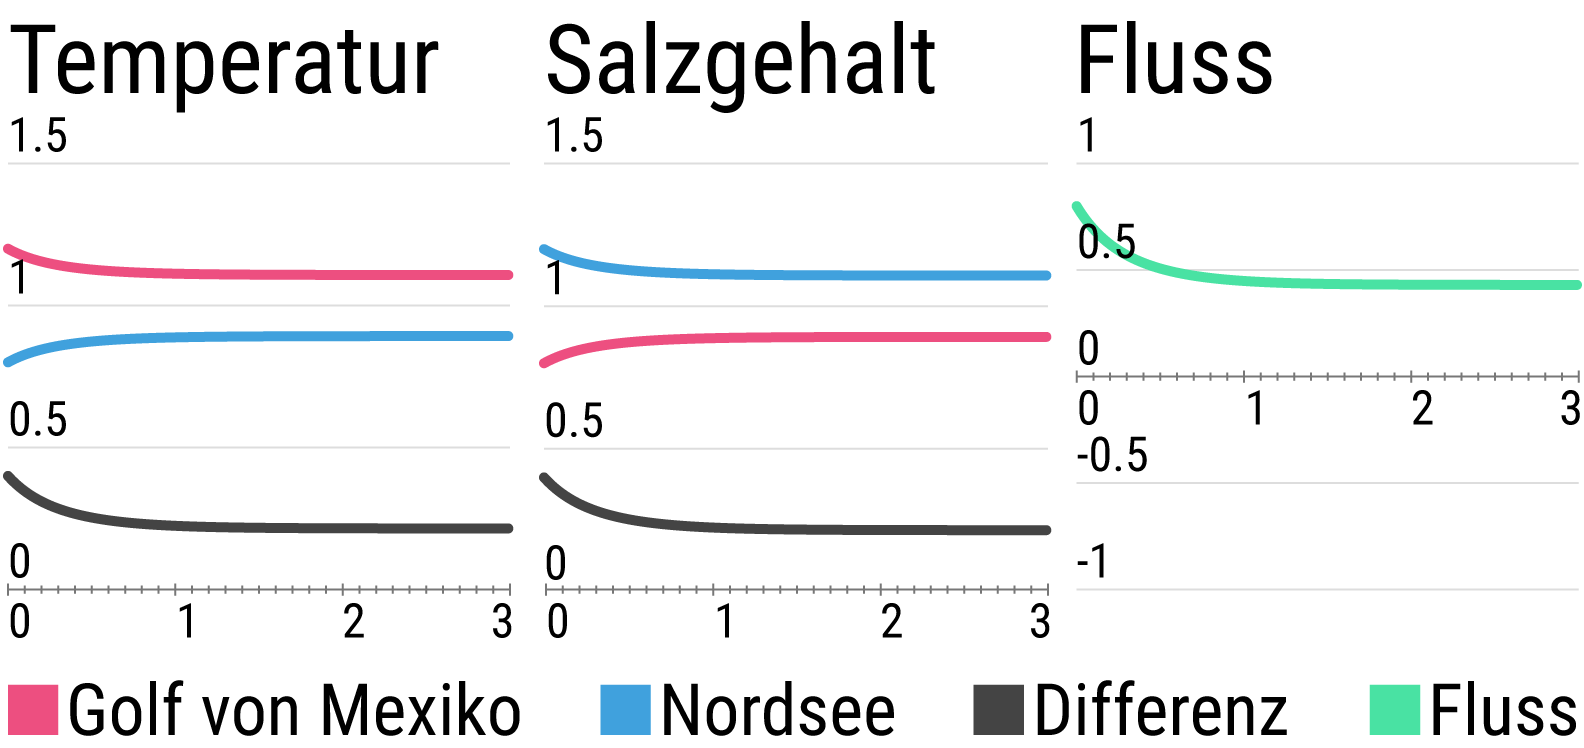
\includegraphics[width=7cm]{../Diagramme/temp-salt-flow_q-pos.png}
  		\caption{Simulation mit folgenden theoretischen Werten \(T_{01} = S_{02} = 1.2, T_{02} = S_{01} = 0.8, k_T = k_S = 1, a = b = c = 1\)}
  		\label{fig:modell_q_pos}
	\end{figure}
	
	Sinkt der Salzgehalt in der Nordsee durch äußere Einflüsse, so ergibt sich ein verändertes Bild. In Abbildung \ref{fig:modell_q_neg} hat der Fluss ein negatives Vorzeichen, er hat sich also umgedreht. Das Wasser fließt neu in entgegengesetzter Richtung von der Nordsee in den Golf von Mexiko.
	\begin{figure}[!h]
  		\centering
 		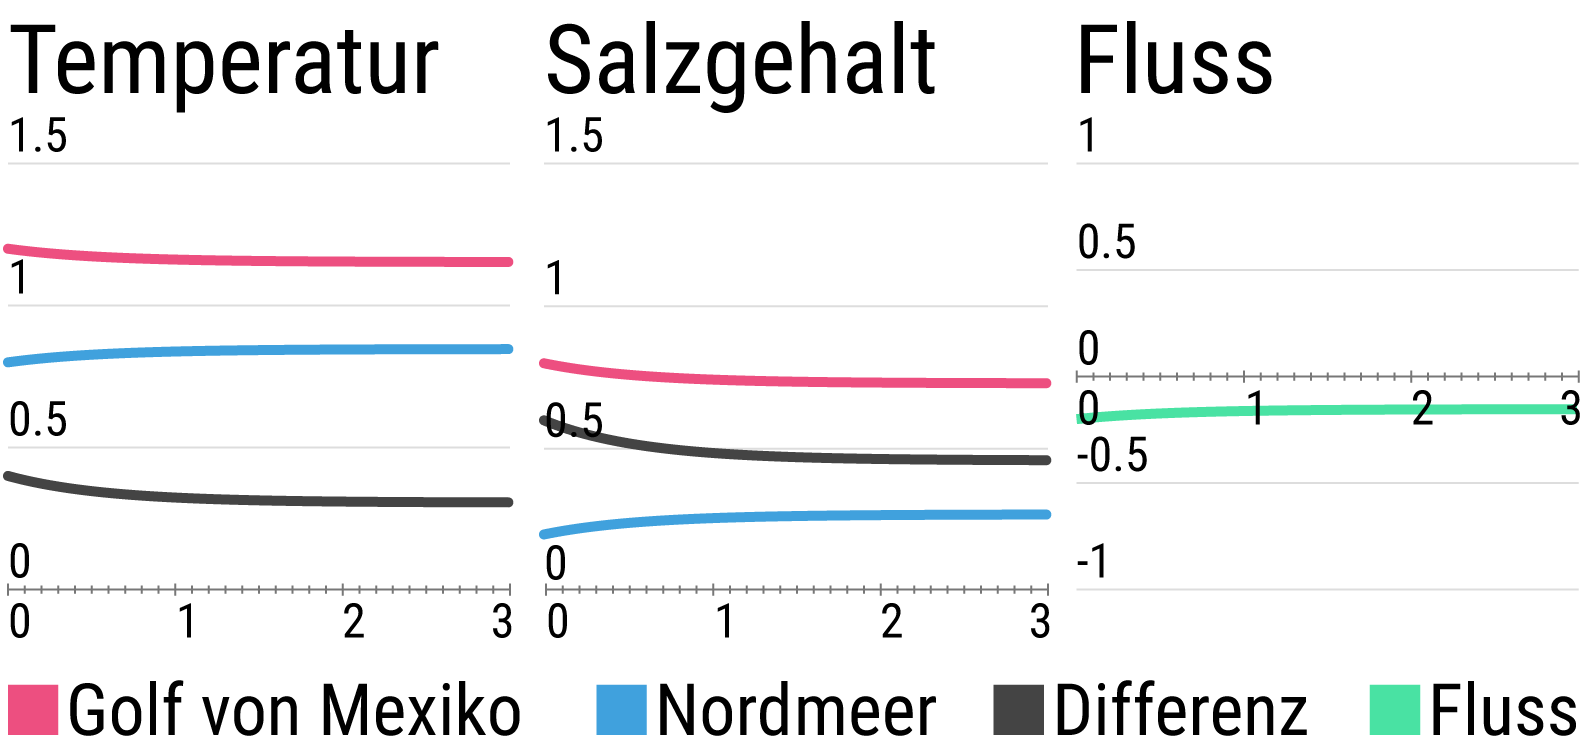
\includegraphics[width=7cm]{../Diagramme/temp-salt-flow_q-neg.png}
  		\caption{Erneute Simulation mit tiefem Salzgehalt \(S_2 = 0.2\) in der Nordsee (die anderen Parameter wurden wie in Abbildung \ref{fig:modell_q_pos} beibehalten)}
  		\label{fig:modell_q_neg}
	\end{figure}
	
	\subsection{Entdimensionalisierung}
	Da die Dimensionen (oder Maßeinheiten) für das Verhalten des Modells keine Rolle spielen, werden diese in einem nächsten Schritt rausgekürzt. Dies geschieht durch die Wahl einer geeigneten Skalierung. Diese ergibt sich, indem wir das Modell nur von dem Verhältnis zu den jeweiligen Startwerten \(T_0, S_0\) abhängig machen. Sei also:
	\begin{align*}
		\tilde{T} = \frac{T}{T_0} \Rightarrow T = \tilde{T} T_0 \quad \textrm{und} \quad \tilde{S} = \frac{S}{S_0} \Rightarrow S = \tilde{S} S_0
	\end{align*}
	
	Eingesetzt in die Gleichung für die Temperaturdifferenz ergibt sich folgendes:
	\begin{align*}
		\frac{d\tilde{T} T_0}{dt} &= k_T\left(T_{0} - \tilde{T} T_0 \right) - 2\left|q(\tilde{T} T_0,\tilde{S} S_0)\right| \tilde{T} T_0 \\
		\stackrel{
			\substack{
				\textrm{da } T_0 > 0\\
				\textrm{ist } T_0 \neq 0
			}
		}{\Rightarrow}
		\frac{d\tilde{T}}{dt} &= k_T\left(1 - \tilde{T}\right) - 2\left|q(\tilde{T} T_0,\tilde{S} S_0)\right| \tilde{T}
	\end{align*}
	Analog gilt für den Salzgehalt:
	\begin{align*}
		\frac{d\tilde{S}}{dt} &= k_S\left(1 - \tilde{S}\right) - 2\left|q(\tilde{T} T_0,\tilde{S} S_0)\right| \tilde{S}
	\end{align*}
	Gilt zusätzlich für den Fluss:
	\begin{align*}
		q = \frac{\tilde{q} k_T}{2} &= a \left( b\tilde{T}T_0 - c\tilde{S}S_0 \right) \\
		\Rightarrow \tilde{q} &= \underbrace{2\frac{ab}{k_T}T_0}_{= \alpha} \cdot \tilde{T} - \underbrace{2\frac{ac}{k_T}S_0}_{=\beta} \cdot \tilde{S} \\
		\Rightarrow \tilde{q} &= \alpha\tilde{T} - \beta\tilde{S}
	\end{align*}
	Skalieren wir zusätzlich noch die Zeit \(t = \tilde{t} k_T\) und setzen \(q = \frac{\tilde{q}k_T}{2}\) ein, so gilt für die Temperatur:
	\begin{align*}
		\frac{d\tilde{T}}{d\tilde{t} k_T} &= k_T\left(1 - \tilde{T}\right) - 2\left|\frac{\tilde{q}(\tilde{T},\tilde{S})k_T}{2}\right| \tilde{T} \\
		\Rightarrow \frac{d\tilde{T}}{d\tilde{t}} &= (1 - \tilde{T}) - \left| \tilde{q}(\tilde{T},\tilde{S})\right|\tilde{T}
	\end{align*}
	Wiederum analog für den Salzgehalt gilt:
	\begin{align*}
		\Rightarrow \frac{d\tilde{S}}{d\tilde{t}} &= \underbrace{\frac{k_S}{k_T}}_{=\gamma}(1 - \tilde{S}) - \left| \tilde{q}(\tilde{T},\tilde{S})\right|\tilde{S}
	\end{align*}
	
	Für die nachfolgende Gleichgewichtsuntersuchung wird nur das dimensionslose Modell betrachtet. Um dafür die Bezeichnungen der Variablen einfach zu halten, wird auf die zusätzliche Notation mit dem \textasciitilde\ verzichtet. Also lauten die dimensionslosen Gleichungen nun:
	\begin{align*}
		\frac{dT}{dt} &= (1 - T) - \left| q(T,S)\right|T \\
		\frac{dS}{dt} &= \gamma (1 - S) - \left| q(T,S)\right|S \\
		q(T,S) &= \alpha T - \beta S
	\end{align*}
	Dafür wurden folgenden Parameter definiert:
	\begin{align*}
		\alpha = 2\frac{ab}{k_T}T_0 \qquad
		\beta = 2\frac{ac}{k_T}S_0 \qquad
		\gamma = \frac{k_S}{k_T}
	\end{align*}
	
	\subsection{Gleichgewichtsuntersuchung}
	Das System ist im Gleichgewicht, wenn sich Temperatur und Salzgehalt nicht mehr ändert:
	\begin{align*}
		\frac{dT}{dt} = (1 - T) - \left| q(T,S)\right|T &\stackrel{!}{=} 0 \\
		\Rightarrow 1 - T(1 + |q|) &\stackrel{!}{=} 0 \\
		\Rightarrow T &= \frac{1}{1 + |q|} \\
		\stackrel{
			\substack{
				\textrm{analog für den}\\
				\textrm{Salzgehalt}
			}
		}{\Rightarrow} S &= \frac{\gamma}{\gamma + |q|}
	\end{align*}
	Damit ist der Fluss:
	\begin{align*}
		q = \alpha \frac{1}{1 + |q|} - \beta \frac{\gamma}{\gamma + |q|} = g(q)
	\end{align*}
	Diesen Zusammenhang bezeichnen wir für die weiteren Untersuchungen als Funktion \(g(q)\).
	
	Wenn sich der Fluss nicht mehr ändert, also stabil ist, muss für \(g(q)\) folgendes gelten:
	\begin{align*}
		g(q) \stackrel{!}{=} q \Rightarrow q - g(q) \stackrel{!}{=} 0
	\end{align*}
	Um also den Fluss im stabilen Zustand zu bestimmen, müssen entsprechende Nullstellen gefunden werden. Im Fall \(\gamma = 1\) und \(q \neq 0\) können die Nullstellen direkt ausgerechnet werden:
	\begin{align*}
		g(q) = q - \frac{1}{1 + |q|}  \left(\alpha - \beta\ \right) &\stackrel{!}{=} 0 \\
		\Rightarrow \frac{q \left( 1 + |q| \right)}{1 + |q|} + \frac{\beta - \alpha}{1 + |q|}  &\stackrel{!}{=} 0 \\
		\stackrel{\textrm{da } 1 + |q| > 0}{\Rightarrow} \left. \begin{array}{ll}
			q > 0: & q^2 + q + \beta - \alpha \\
			q < 0: & -q^2 - q + \beta - \alpha
		\end{array} \right\} &\stackrel{!}{=} 0 \\
		\Rightarrow \begin{array}{l}
			q > 0 \left\{ \begin{array}{l}
				q_1 = \frac{1}{2}\left( -\sqrt{4a - 4b + 1} -1 \right)	\\			
				q_2 = \frac{1}{2}\left( +\sqrt{4a - 4b + 1} -1 \right)				
			\end{array}\right. \\
			q < 0 \left\{ \begin{array}{l}
				q_3 = \frac{1}{2}\left( -\sqrt{4b - 4a + 1} + 1 \right) \\
				q_4 = \frac{1}{2}\left( +\sqrt{4b - 4a + 1} + 1 \right)
			\end{array}\right.
		\end{array}
	\end{align*}
	Da \(q_1\) für reelle Werte die Bedingung \(q > 0\) nicht erfüllt, kann es keine Nullstelle sein. Auch \(q_4\) kann für reelle Werte die Bedingung \(q < 0\) nicht erfüllen. Also verbleiben für den Fall \(\gamma = 1\) die Nullstellen \(q_2\) und \(q_3\).
	
	\begin{figure}[!h]
  		\centering
 		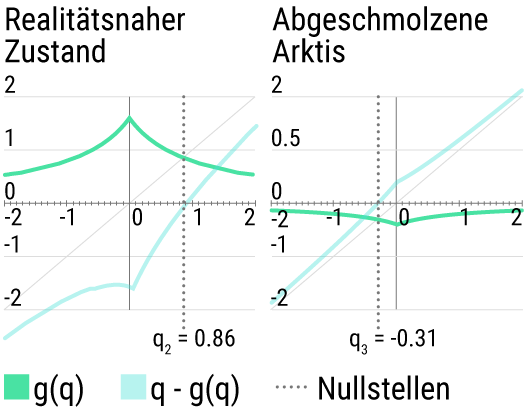
\includegraphics[width=6cm]{../Diagramme/g_von_q_gamma_1.png}
  		\caption{Die Funktion \(g(q)\) mit den Nullstellen \(q_2\) und \(q_3\) für die bereits beschriebenen Werte im realitätsnahen Zustand (siehe Abbildung \ref{fig:modell_q_pos}) und im Fall einer abgeschmolzenen Arktis (siehe Abbildung \ref{fig:modell_q_neg}).}
  		\label{fig:g_von_q_gamma_1}
	\end{figure}	

	
	Um auch den Fall \(\gamma \neq 1\) betrachten zu können, wird die Funktion \(g(q)\) so erweitert, dass die Brüche wegfallen aber die Nullstellen erhalten bleiben:
	\begin{align*}
		k(q) = \left\{ \begin{array}{ll}
			\left( q - g\left(q\right) \right)(1 + q)(\gamma + q) &\textrm{ für } q > 0  \\
			\left( g\left(q\right) - q \right)(1 - q)(\gamma - q) &\textrm{ für } q < 0
		\end{array} \right.
	\end{align*}
	Aufgrund der Betragsfunktion für \(q\) in der Funktion \(g(q)\) müssen wir die Fälle \(q > 0\) und \(q < 0\) getrennt betrachten. Im weiteren wird der Fall \(q > 0\) besprochen, der Fall \(q < 0\) folgt analog.
	
	Eingesetzt und ausmultipliziert ergibt sich folgendes Polynom:
	\begin{align*}
		k(q) &= q^3 + q^2(1 + \gamma) + q\left(\gamma \left(1 + \beta\right) - \alpha \right) + \gamma \left( \beta - \alpha \right)
	\end{align*}
	Die Funktion \(k(q)\) ist ein Polynom 3ten Grades und hat höchstens drei Nullstellen. Diese drei Nullstellen müssen wiederum zwei Wendepunkte einschließen. Die Wendepunkte werden wie folgt gefunden:
	\begin{align*}
		k'(q) &= 3q^2 + 2q(1+\gamma) + \gamma(1+\beta) - \alpha \stackrel{!}{=} 0 \\
		\Rightarrow& \left\{ \begin{array}{l}
			q_{w1} = -\frac{1}{3}\left( \sqrt{3\alpha - 3\beta\gamma + \gamma^2 - \gamma + 1} +\gamma + 1 \right) \\
			q_{w2} = \frac{1}{3}\left( \sqrt{3\alpha - 3\beta\gamma + \gamma^2 - \gamma + 1} -\gamma - 1 \right)
		\end{array} \right.
	\end{align*}
	Der Wendepunkt \(q_{w1}\) kann für reelle Punkte nicht größer Null sein, also hat \(k(q)\) für \(q > 0\) nur den Wendepunkt \(q_{w2}\) und kann somit auch nur zwei Nullstellen im Bereich \(q > 0\) haben.
	
	Gilt \(k(q_{w2}) = 0\) so ist gerade der Wendepunkt ein Nullpunkt und die Funktion \(k(q)\) hat eine Nullstelle für \(q > 0\).
	
	Ist \(k(0) > 0\) und \(k(q_{w2}) > 0\) so existiert für \(q > 0\) keine Nullstelle, so beispielsweise im Fall der abgeschmolzenen Arktis.
	
	
	\section{\uppercase{Anwendung}}\label{sec:Anwendung}
	\noindent Nach der theoretischen Analyse wollen wir unser Modell welches noch nicht enddimensioniert wurde betrachten. Dazu haben wir recherchiert und die tatsächlichen Temperaturen des Golfstrom genommen. Da sich die Quellen jedoch unterscheiden, da in verschieden Tiefen gemessen wurde oder zu verschieden Jahreszeiten oder die Genauigkeit der Messung variiert haben wir uns dazu entschieden ein Mittel der Werte zu nehmen.
	
	\subsection{Datenabschätzung} \label{Datenabschaetzung}
	\noindent Betrachten wir nun zuerst die Temperaturen des Golfstromes im Golf von Mexiko. Der Golf von Mexiko hat eine durchschnittliche Temperatur von ungefähr 27 Grad Celsius. An manchen Küstenabschnitten etwas wärmer an anderen etwas kühler. An der Küste wird der Golfstrom in seinem Fluss gestört, da dort der Meeresgrund nicht überall gleich tief ist. So kommt es dazu, dass der Fluss an mancher Stelle durch eine enge muss und sich somit die Fließgeschwindigkeit erhöht und an andere Stelle wird er wieder gebremst. Dadurch verweilt die Wassermenge an einer Stelle länger und wird stärker von der Sonne erwärmt. 
	
	Die Temperatur vom Nordmeer haben wir mit rund 10 Grad Celsius angenommen. Hierbei ist es schwer, da das Nordmeer relativ groß ist und sich über circa 15 Breitengrade erstreckt. Das ist eine Länge von über 2000 Kilometern. Auf dieser enormen Länge schwankt die Temperatur erwartungsgemäß stark. Das südliche Ende liegt westlich von Norwegen ungefähr auf dem 60. Breitengrad. Das nördliche Ende ist ungefähr bei dem 75. Breitengrad. Das ist deutlich oberhalb des Polarkreises (66.5 Breitengrad; Island liegt ungefähr auf dem Polarkreis).

	Erstaunlicher weiße haben wir sehr gute Wetterdiagramme auf Reiseseiten gefunden. Dort wird oft aufgelistet, wann die beste Reisezeit ist und es werden einem erstaunlich gute Graphiken gezeigt die sowohl die Umgebungstemperatur als auch die Wassertemperatur liefen. Da diese Diagramme meist kein Quellenverzeichnis aufweisen, haben wir die Werte mit anderen Messdaten "validiert". Die Abweichungen waren vernachlässigbar gering. Aus diesen Diagrammen kann man sich nun ein sehr detailliertes Bild machen, wie sich die Wassertemperatur entlang der Küste verändert, da es zu jedem größeren Küstenort ein solches Diagramm gibt.

	Beim Salzgehalt gestaltet sich die Suche nach brauchbaren Werten jedoch deutlich schwerer. Zum Nordmeer findet man mehr Messerwerte über den Salzgehalt, da dort das Wasser aufgrund der Kombination von Salz und Frost dichter wird und nach unten sinkt. Der Durchschnittswert der Salinität beträgt hier um die 34 Promille. 

	Im Golf von Mexiko findet man so gut wie keine Werte. Deshalb können wir hier nicht sonderlich vergleichen. Die Salinität liegt hier bei 31 bis 32 Promille.

	Diese Werte haben wir in unser Simulink Modell des Golfstromes eingefügt. Es stellt sich jedoch die Frage, ob wir die gemessenen Werte nun tatsächlich die Umgebungstemperaturen sind, oder ob die Werte die Temperaturen vom Golfstrom sind. Schaut man sich die Auswirkungen des Golfstrom an wird deutlich, das er im Norden das Wasser erwärmt und im Süden kühlt. Also müssen die Umgebungstemperaturen im Norden niedriger und im Süden größer sein, als die Temperatur des Golfstroms. Da wir nicht wissen wie stark die Temperatur des Golfstromes von der Umgebung beeinflusst wird und anders herum gestaltet sich die Wahl der richtigen Werte sehr schwer. Wir haben deshalb die Temperatur des Golfstrom auf eine Wert gebracht der im Süden niedriger ist als die tatsächliche Temperatur und die Umgebungstemperatur wärmer als die tatsächliche Temperatur. Im Norden haben wir dies genau anders herum gemacht, da dort der Golfstrom erwärmt und somit wärmer sein muss als die Umgebung.
	
	In unserem Modell wird nur die Auswirkung der Umgebungstemperatur betrachtet, da eine Rückwirkung noch mehr Messwerte benötigen würde, welche uns nicht zugänglich sind.  
	

	\subsection{Die Arktis schmilzt} \label{dieArktisSchmilzt}
	
	Aufgrund des Klimawandels erhöht sich die Temperatur weltweit. So auch Nördlich des Polarkreises. Wir haben diese Temperaturerhöhung in unserem Modell umgesetzt. Dazu haben wir die Umgebungstemperatur T02 von der Zeit abhängig gemacht. Das heißt wir haben die Temperatur doch ein logistisches Wachstum beschrieben. Wir starten mit der Umgebungstemperatur für die Wir wissen, dass wir eine Gleichgewichtsbedingung haben und erhöhen diesen Wert dann gegen eine obere Grenze. Wenn sich die Temperatur erhöht beginnt natürlich auch das Eis zu schmelzen.
		
	Beim Schmelzen der Arktis wird viel Wasser, welches in gefrorenem Zustand als Süßwasser vorliegt zusätzlich in das Nordmeer gelangen. Dadurch wird der Salzgehalt im Nordmeer abnehmen, da sich das Salz auf mehr Wassermenge verteilen wird. Dies haben wie umgesetzt, indem wir den Umgebungssalzgehalt S02 durch einen logarithmischen Zerfall beschrieben haben. Das heißt der Salzgehalt sinkt mit der Zeit auf einen niedrigeren Wert. 
	
	\begin{figure}[!h]
  		\centering
 		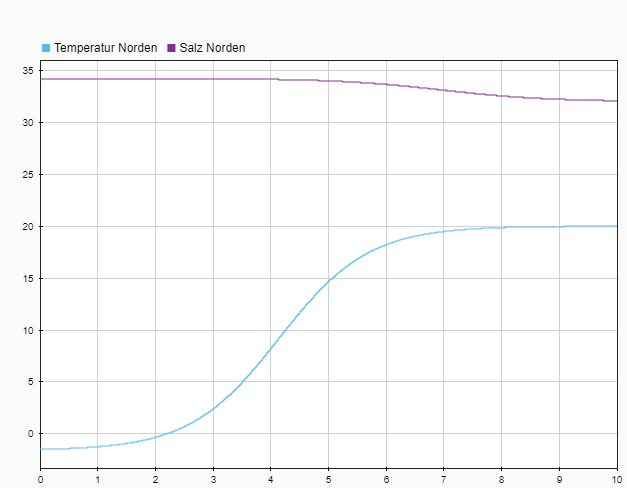
\includegraphics[width=7cm]{../Diagramme/Arktis_schmilzt_init.png}
  		\caption{Werte mit denen der Golfstrom angeregt wird}
  		\label{fig:schmilztUmgebung}
	\end{figure}

	Man sieht deutlich, dass sich die Temperatur des Golfstromes im Norden auch erhöht. Die Kurve von T2 (Temperatur des Golfstroms im Norden) sieht ähnlich aus wie die Kurve der Umgebungstemperatur T02 mit der sie angeregt wird. Dies ist sehr gut nachvollziehbar, da T02 sich direkt auf T2 auswirkt. Erstaunlich ist dass sich auch die Temperatur vom Golfstrom im Süden erhöht. Dies ist jedoch bei genauerer Betrachtung auch logisch. Die Temperatur im Süden vom Golfstrom wird direkt von der Temperatur im Norden beeinflusst. Kommt von Norden wärmeres Wasser, so wird das Wasser im Süden nicht so stark gekühlt und gleicht sich mehr der Umgebungstemperatur im Süden an.
	
	Beim Salz folgt es genau der gleichen Schema, da Salz und Temperatur jeweils von äquivalenten Gleichungen beschrieben werden. Auch hier sinkt der Salzgehalt im Norden und der Salzgehalt im Süden vom Golfstrom nimmt mit ab.

	\begin{figure}[!h]
  		\centering
 		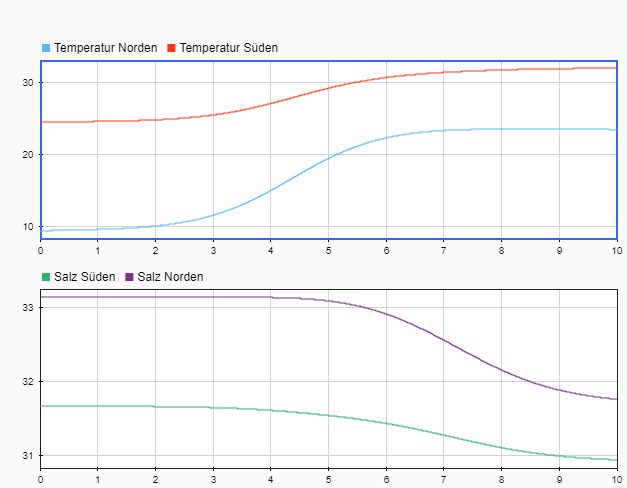
\includegraphics[width=7cm]{../Diagramme/Arktis_schmiltz_werte.png}
  		\caption{Auswirkungen auf den Golfstrom}
  		\label{fig:schmilztGolf}
	\end{figure}

	\subsection{Temperaturschwankungen durch Jahreszeiten} \label{TempDurchJahreszeiten}
	
	Als nächstes stellt sich die Frage ob und wie Stark sich die Schwankung der Temperatur über ein Jahr auf den Fluss des Golfstroms auswirkt. Dazu haben wir Klimadiagramme vom Nordmeer und vom Golf von Mexiko heran gezogen und diese durch einen Sinus nachgeahmt. 
	
	Im Golf von Mexiko schwingt die Temperatur über ein Jahr um circa 11 Grad Celsius. Das Maximum liegt hier bei rund 30 Grad Celsius Wassertemperatur welche im Juli erreicht wird. Im Januar ist die Wassertemperatur mit rund 19 Grad am niedrigsten.
	
	Die Temperatur schwingt im Nordmeer nur um circa 3 Grad Celsius. Auch hier werden die kältesten Temperaturen im Januar und Februar gemessen. Diese betragen 4 bis 6 Grad Celsius. Die wärmste Temperatur wird im Juli und August gemessen. 
	
	Aufgrund von diesen Werten haben wir eine Anregung der Umgebungstemperatur vom Golf von Mexiko T01 und vom Nordmeer T02 in Abhängigkeit von der Zeit entworfen. Da an beiden Orten die Temperaturextreme etwas zur gleichen Zeit auftreten arbeiten wir jeweils mit der selben Phasenverschiebung. 
	
	\begin{figure}[!h]
  		\centering
 		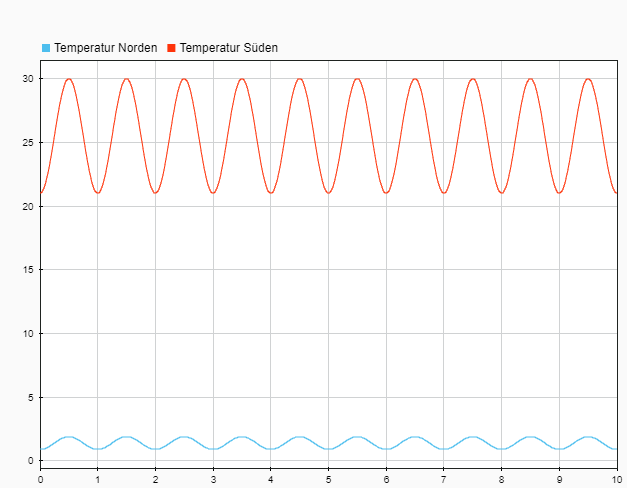
\includegraphics[width=7cm]{../Diagramme/Jahreszeiten_init.png}
  		\caption{Werte mit denen der Golfstrom angeregt wird}
  		\label{fig:jahreszeitenUmgebung}
	\end{figure}
	
	Wie wir bereits in \ref{dieArktisSchmilzt} gesehen haben, wirkt sich die Umgebungstemperatur direkt auf die Temperatur des Golfstromes aus. Die Temperaturen des Golfstromes nehmen sehr schnell die Schwingungen an. Auffällig ist, das es am Anfang eine starken Abfall gibt. Dieser kommt jedoch daher, das wir durch die Schwingung nicht mehr in unserem Gleichgewichtspunkt starten. Deshalb ist dieser starke Abfall zu vernachlässigen. Danach schwingen die Temperaturen weiter um einen stabilen Punkt und weichen nicht mehr davon ab. Wir kommen deshalb zu der Erkenntnis, dass sich auch die Jahreszeiten auf den Golfstrom auswirken. Betrachtet man den Fluss so stellt man fest, dass dieser ebenfalls schwingt. Im Sommer fließt der Golfstrom schneller als im Winter. Dies sieht man direkt, wenn man sich die Gleichung für den Fluss anschaut, da dieser abhängig ist von der Differenz der Temperaturen im Norden und Süden. Da die Temperatur im Norden weniger stark schwingt als die Temperatur im Süden wird im Winter eine kleiner Differenz erreicht und damit wird der Fluss geringer.
	
	Der Salzgehalt fängt ebenfalls an zu schwingen. Dies liegt daran, dass sie Temperatur und Salzgehalt gegenseitig beeinflussen. Das Salz schwingt jedoch nur in einem sehr kleinen Bereich und spielt dadurch fast keine Rolle.

	\begin{figure}[!h]
  		\centering
 		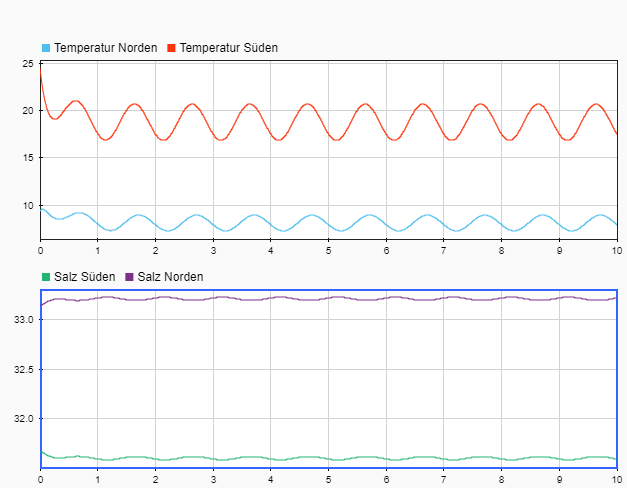
\includegraphics[width=7cm]{../Diagramme/Jahreszeiten_werte.png}
  		\caption{Auswirkungen auf den Golfstrom}
  		\label{fig:jahreszeitenGolf}
	\end{figure}

	\section{\uppercase{Fazit}}\label{sec:Fazit}
	
	Wir wollen uns nun der Frage stellen, ob  der Golfstrom zum Erliegen kommen wird. Um die Fragestellung zu beantworten betrachten wir das Modell das wir in \ref{dieArktisSchmilzt} benutzt haben, da wir in \ref{TempDurchJahreszeiten} festgestellt haben, dass die Jahreszeiten keine Auswirkung auf die Gleichgewichtspunkte haben sondern nur um diese Schwingen. Es könnte sein, dass durch eine solche Schwingung das erliegen des Golfstromes etwas früher eintreten könnte jedoch wollen wir dies vernachlässigen.
	
	Durch Simulation mit mehreren Werten hat sich herausgestellt, dass die Umgebungstemperatur im Norden auf 29 Grad Celsius erhöhen müsste. Das würde bedeuten dass der Golfstrom eine Temperatur von fast 30 Grad Celsius annehmen würde. Des Salzgehalt im Norden müsste auf 29.7\% abfallen. 
	
	Laut unserem Modell sind wir also noch ziemlich weit von einem stillstand des Golfstromes entfernt. 
	
	Es sollte jedoch klar sein, dass sich der Golfstrom nicht durch ein derart einfache Modell beschreiben lässt. Es mussten zu viele Vereinfachungen getroffen werden, dass die Aussagekraft unseres Modells stark begrenzt ist. 
	
	Der Fluss wurde sehr stark vereinfacht indem er als zwei Pipelines dargestellt wurde. In echt ist der Fluss jedoch viel komplexer. Es findet ein Austausch zwischen den beiden statt, da sie in der Realität direkt aneinander vorbei fließen. So kann Wasser von dem einen Fluss in den anderen Fluss gelangen und die Temperatur auf der Reise verändert werden welche von uns nicht berücksichtigt wurde. Zum anderen spielt die Fluiddynamik eine Rolle. Nicht nur dass sich die beiden Flüsse in ihrer Geschwindigkeit gegenseitig bremsen wird auch noch durch die Beschaffenheit des Meeresbodens der Fluss des Golfstromes beeinflusst. Auch ist der Weg vom Golf von Mexiko ins Nordmeer länger als der Rückweg, da nicht beides mal der selbe Weg genommen wird.
	
	Wie in \ref{Datenabschaetzung} bereits angesprochen wurde, wird die Auswirkung des Golfstromes auf die Umgebung nicht berücksichtigt obwohl dies eine sehr wichtige Rolle spielt. Es gibt auch eine Wechselwirkung zwischen Golfstrom und dem Windsystem. Wie in \ref{sec:Golfstrom} beschrieben spaltet sich ein Teil des Wasser vom Golfstrom ab und fließt wieder zurück in Richtung des Äquators. Genau über diesem Zyklus kann man auch einen Kreisbewegung im Windsystem feststellen
	
	Auch ist es falsch den Golfstrom als abgeschlossenes System mit einem Behälter für den Golf von Mexiko und eine für das Nordmeer zu sehen, da andere Meeresströmungen ebenfalls Einwirkungen haben und anderen wiederum vom Golfstrom Energie beziehen und dadurch angetrieben werden.
	
	Trotzdem macht das Modell Sinn um einen Einblick in das Verhalten des Golfstromes zu bekommen. Eine Qualitative Aussage ist mit diesem Modell durchaus möglich. Jedoch macht es wenig Sinn zu versuchen mit realen Werten zu arbeiten. 
	
 	\section{\uppercase{Quellen}}\label{sec: Quellen}

	Golf von Mexiko
	\begin{verbatim}
	https://de.wikipedia.org/wiki/Salinit%C3%A4t#/media/File:WOA09_sea-surf_SAL_AYool.png
	\end{verbatim}		
	
	Dokumentationen über dem Golfstrom: 
	\begin{verbatim}
		https://www.youtube.com/watch?v=cV4tC9plmZs&feature=youtu.be
		https://www.youtube.com/watch?v=kuUgHZXkLNU&t=9s
		https://www.youtube.com/watch?v=yKXiNJ4mQ3M
  	\end{verbatim}		
	Sonstiges: 
	\begin{verbatim}
		https://data.giss.nasa.gov/
		https://en.wikipedia.org/wiki/Sea_surface_temperature
	\end{verbatim}
	
	\nocite{*}
	\bibliographystyle{acm}
	\bibliography{Quellen}

\end{document}	

